\documentclass{article}
\usepackage{nott-titlepage}
\usepackage{graphicx}
\usepackage{pdfpages}
\usepackage{float}
\usepackage{hyperref}
\usepackage{tabularx}
\bibliography{main.bib}

\title{Power Electronics Coursework 1 Report}
\author{Tan Hong Kai}
\date{April, 5 2024}
\studentid{20386501}
\module{EEEE3112 Power Electronic Applications and Control}
\department{Department of Electrical and Electronics Engineering}

\includepdfset{pages=-}

\begin{document}
\maketitle

\section{Introduction}

This coursework explores designing a DC/DC converter for the application of CPU.
Designing a good power electronics converter for a CPU becomes important as new generation CPU requires more stringent power input.
In this coursework a DC/DC converter for a CPU with requirements shown in table \ref{tab:cpu-requirement} is designed.

\begin{table}[ht]
    \label{tab:cpu-requirement}
    \caption[Design Requirements]{Design Requirements for CPU}
    \centering
    \begin{tabular}{| l | l | l |}
        \hline
        Specification/Term                         & Symbol                 & Value         \\
        \hline
        DC Supply Voltage                          & $V_{DC}$               & 5 V           \\
        Output Voltage                             & $\bar{V}_{BN}$/$V_{o}$ & 1.8 V         \\
        Output Current                             & $I_{o}$                & 18 A          \\
        Switching frequency                        & $f_s$                  & 200 kHz       \\
        Output voltage ripple                      & $\Delta{}V_o$          & 1 mV          \\
        Internal resistance of the filter inductor & $R_L$                  & 5 m$\Omega$   \\
        ESR of the filter capacitor                & ESR                    & 0.05 $\Omega$ \\
        \hline
    \end{tabular}
\end{table}

\subsection{Assumptions}

Assumptions and decisions needed are made for the calculation of the components value.

For the design of the power supply, current ripple of 25\% of output current is considered.
A Current ripple too small will cause size of the inductor to be big, but it shouldn't be too high to break the CPU.
According to Intel ATX specification, the maximum output current ripple should be 30\%. \cite{intel-design-guide}
However, just to allow for some margin for unknown factors during the building of the power supply that effect current ripple a value of 25\% of current output is chosen.

Another assumption made during the design process of the converter is the resistance value of the CPU.
For the design of converter, the CPU is assumed to be a purely resistive load $R$ of $0.1 \Omega$

Lastly, decisions are made for what components used for the transistor and diodes.
This will affect the losses in the circuit when simulating with losses.
For the transistor, the IQE004NE1LM7CGSC MOSFET from Infineon is chosen for this application.
It can handle up to 379 A, with small turn on resistance.
For the diode in unidirectional design, the 1N5817 Schottky diode.
A Schottky diode is chosen due to its low forward bias voltage and high switching speed.

From the data sheet of the components, some loss values needed for loss simulation can be obtained:

\begin{itemize}
    \item Transistor turn-on resistance: $R_{son} = 0.45 m\Omega$
    \item Diode forward voltage drop: $V_{f} = 0.45 V$
    \item Diode turn on resistance: $R_{don} = 0.45 \Omega$
\end{itemize}

Note: The diode turn on resistance can be obtained by using the \hyperref[fig:IV-curve-diode]{I-V curve}.

\begin{figure}[ht]
    \centering{}
    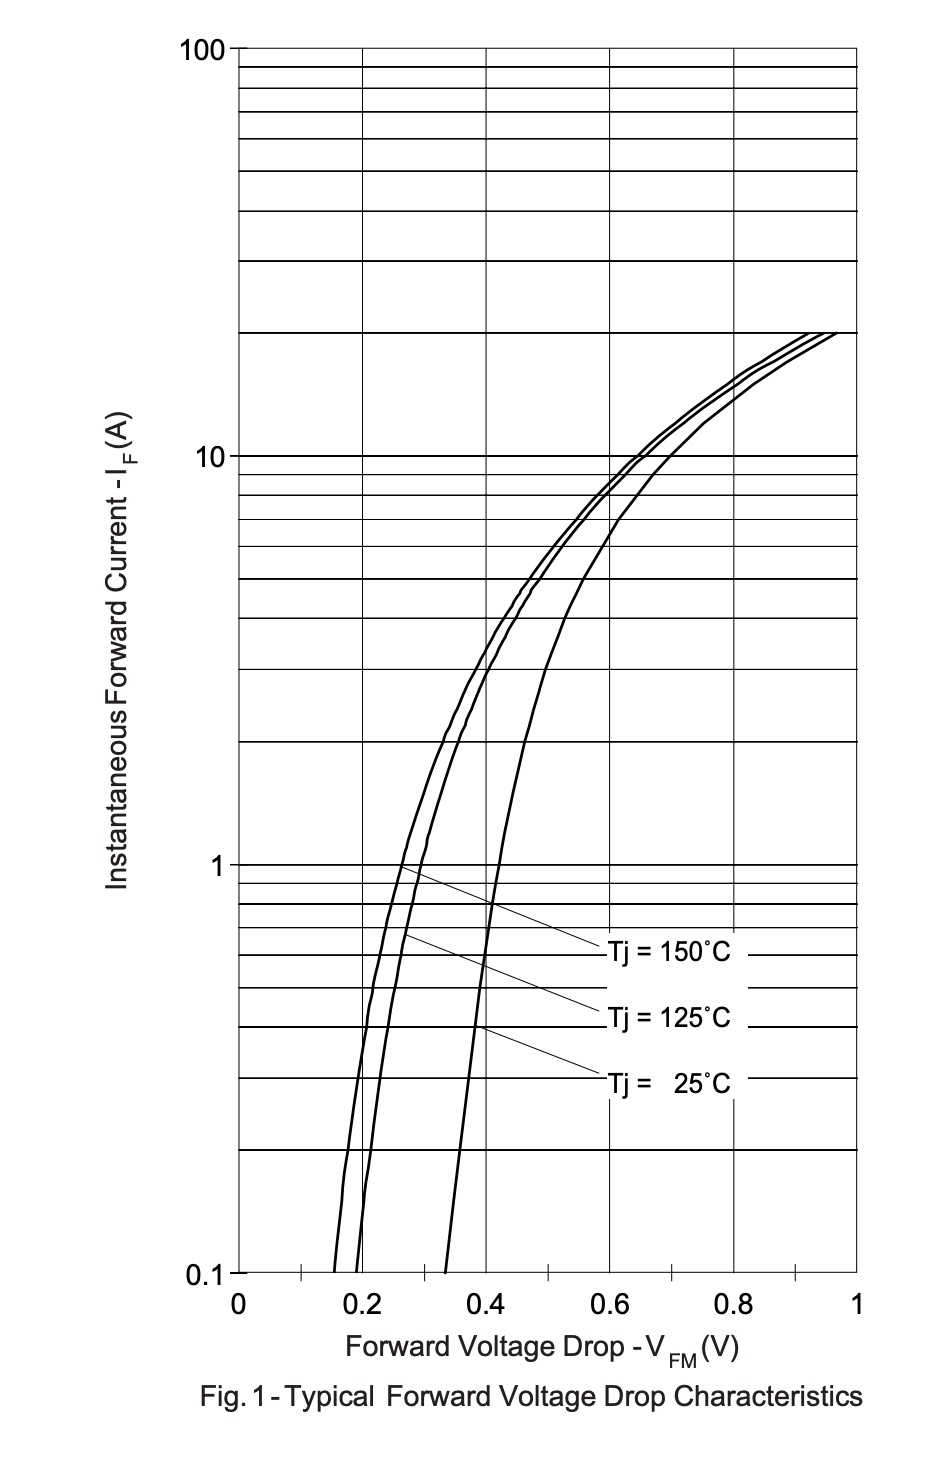
\includegraphics[height=0.5\textheight]{img/I-V-plot.jpg}
    \label{fig:IV-curve-diode}
    \caption{I-V curve for 1N5817}
\end{figure}

\section{Components Calculation}

\subsection{Design Parameters}

$\Delta{}V = 1 mV$

$f_s = 200 kHz$

$T_s = 1 / f_s = 5 \mu{s}$

$V_{DC} = 5 V$

$V_o = 1.8 V$

$I_o = 18 A$

$m = V_0 / V_{DC} = 0.36$

$\Delta{I} = 25\% I_o = 4.5 A$

$R = 0.1 \Omega$

\subsection{Filter Inductor}

$L = \frac{V_{DC} (1 - m) m T_s}{\Delta{I}} = 1.28 \mu{H}$

\subsection{Filter Capacitor}

$C = \frac{T_s \Delta{I}}{8 \Delta{V}} = 2.8 m{F}$

\section{PLECS Circuits}

\subsection{Bidirectional without Losses}

\begin{figure}[H]
    \centering{}
    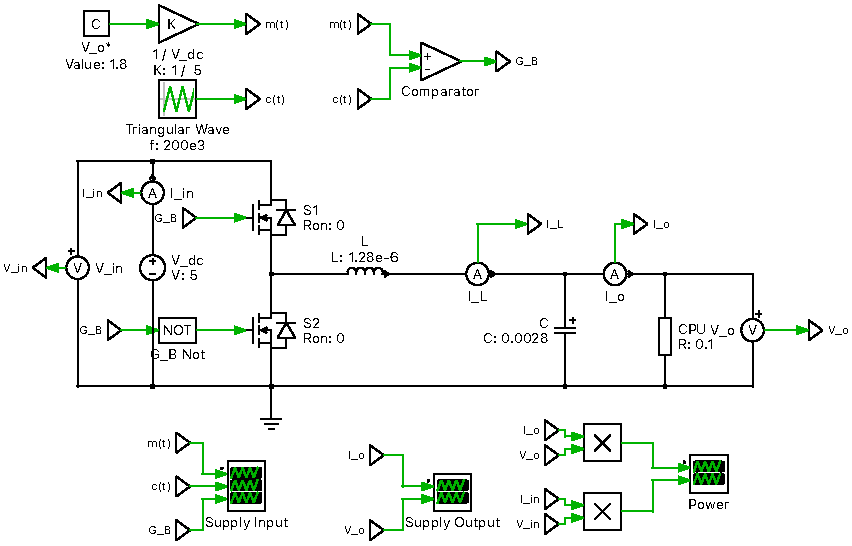
\includegraphics[width=\textwidth]{img/ideal-bidirectional.pdf}
    \label{fig:ideal-bi-circuit}
    \caption{Circuit for Ideal Bidirectional DC/DC Converter}
\end{figure}

\subsection{Unidirectional without Losses}

\begin{figure}[H]
    \centering{}
    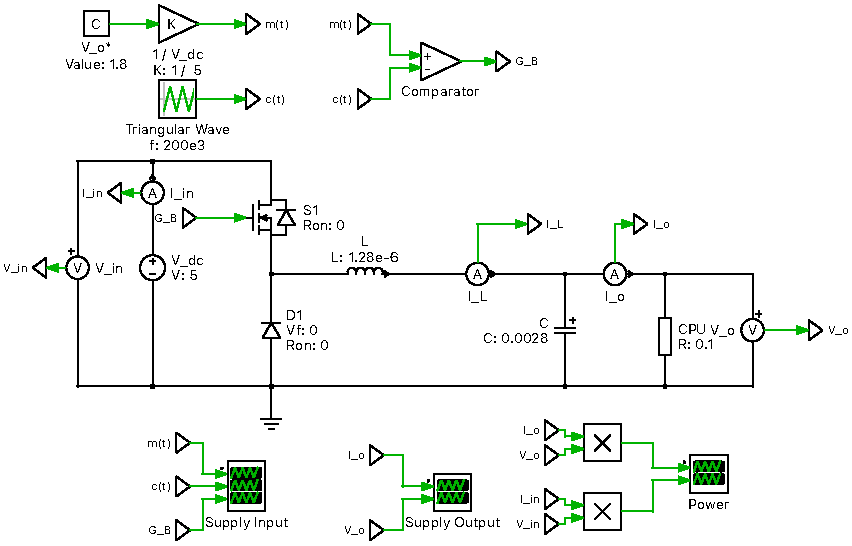
\includegraphics[width=0.8\textwidth]{img/ideal-unidirectional.pdf}
    \label{fig:ideal-uni-circuit}
    \caption{Circuit for Ideal Unidirectional DC/DC Converter}
\end{figure}

\subsection{Bidirectional with Losses}

\begin{figure}[H]
    \centering{}
    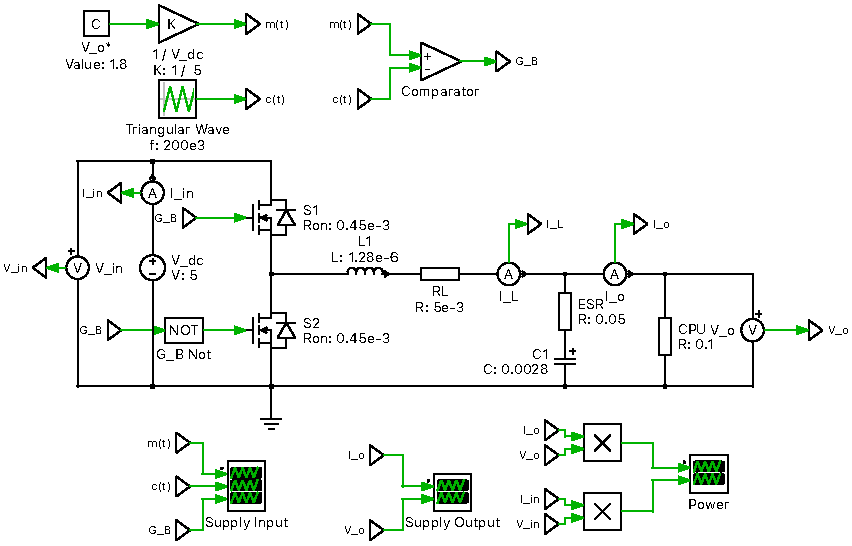
\includegraphics[width=0.8\textwidth]{img/loss-bidirectional.pdf}
    \label{fig:loss-bi-circuit}
    \caption{Circuit for Loss Bidirectional DC/DC Converter}
\end{figure}

\subsection{Unidirectional with Losses}

\begin{figure}[H]
    \centering{}
    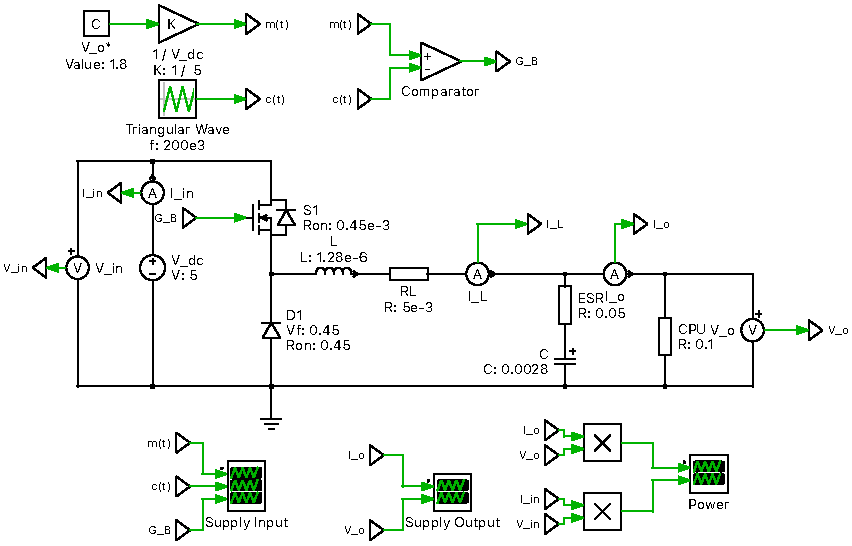
\includegraphics[width=0.8\textwidth]{img/loss-unidirectional.pdf}
    \label{fig:loss-uni-circuit}
    \caption{Circuit for Loss Unidirectional DC/DC Converter}
\end{figure}

\section{Waveforms}

\subsection{Bidirectional without Losses}

\begin{figure}[H]
    \centering{}
    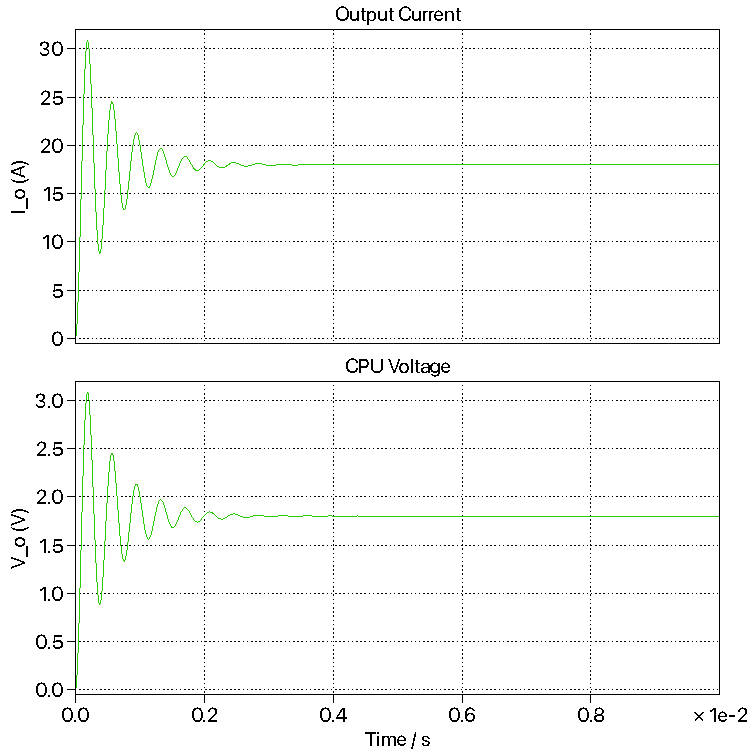
\includegraphics[width=0.6\textwidth]{img/ideal-I-V-bidirectional.pdf}
    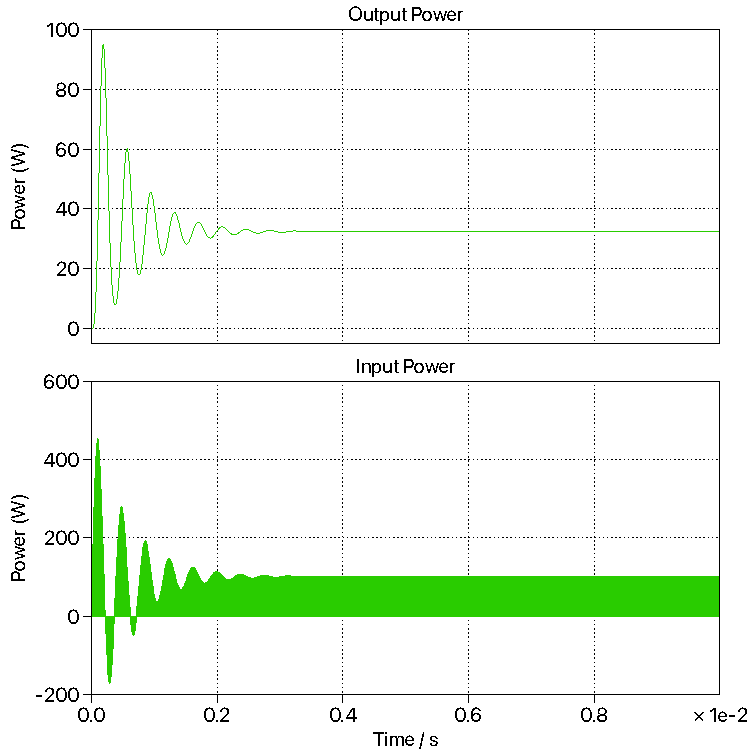
\includegraphics[width=0.6\textwidth]{img/ideal-power-bidirectional.pdf}
    \label{fig:ideal-bi-plots}
    \caption{Current, Voltage and Power Plot for Ideal Bidirectional DC/DC Converter}
\end{figure}

\subsection{Unidirectional without Losses}

\begin{figure}[H]
    \centering{}
    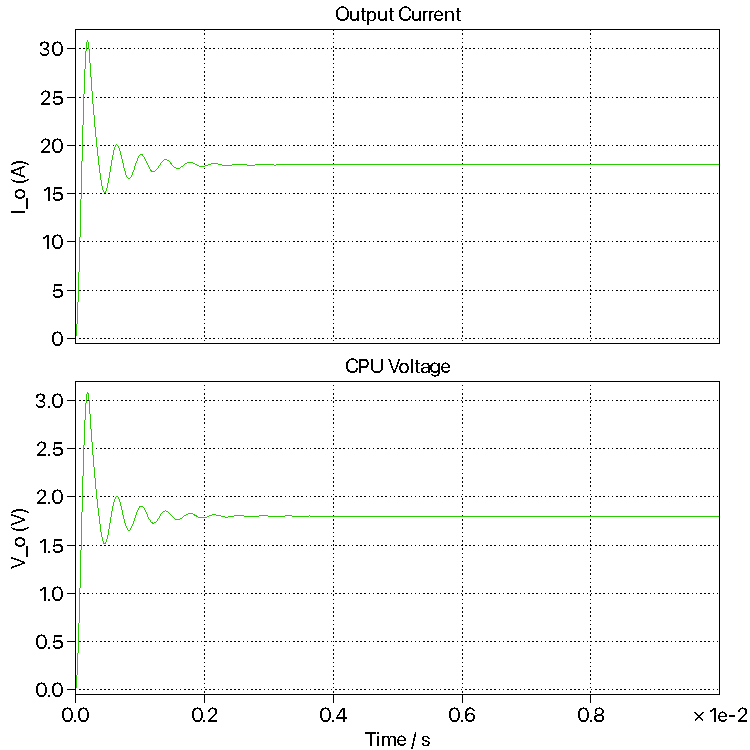
\includegraphics[width=0.6\textwidth]{img/ideal-I-V-unidirectional.pdf}
    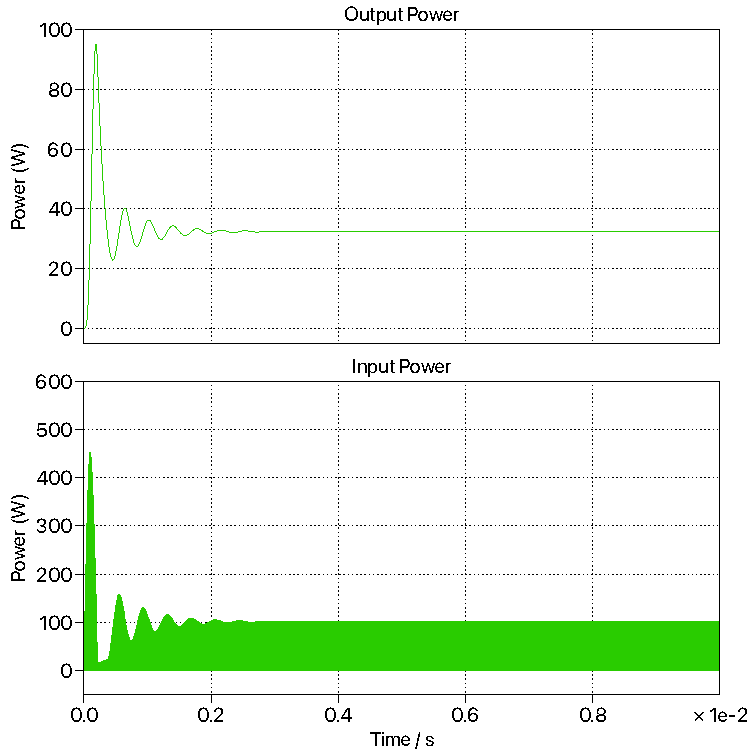
\includegraphics[width=0.6\textwidth]{img/ideal-power-unidirectional.pdf}
    \label{fig:ideal-uni-plots}
    \caption{Current, Voltage and Power Plot for Ideal Unidirectional DC/DC Converter}
\end{figure}

\subsection{Bidirectional with Losses}

\begin{figure}[H]
    \centering{}
    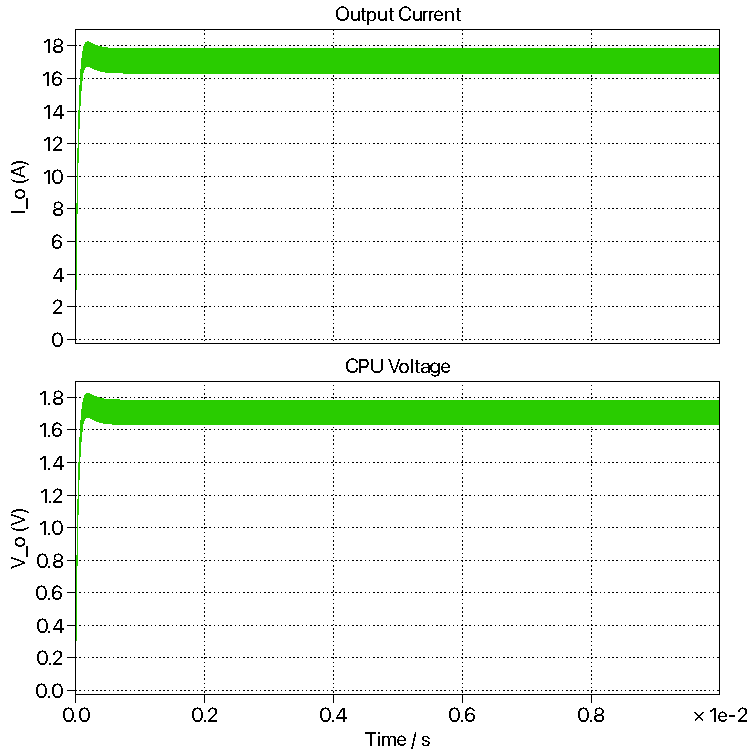
\includegraphics[width=0.6\textwidth]{img/loss-I-V-bidirectional.pdf}
    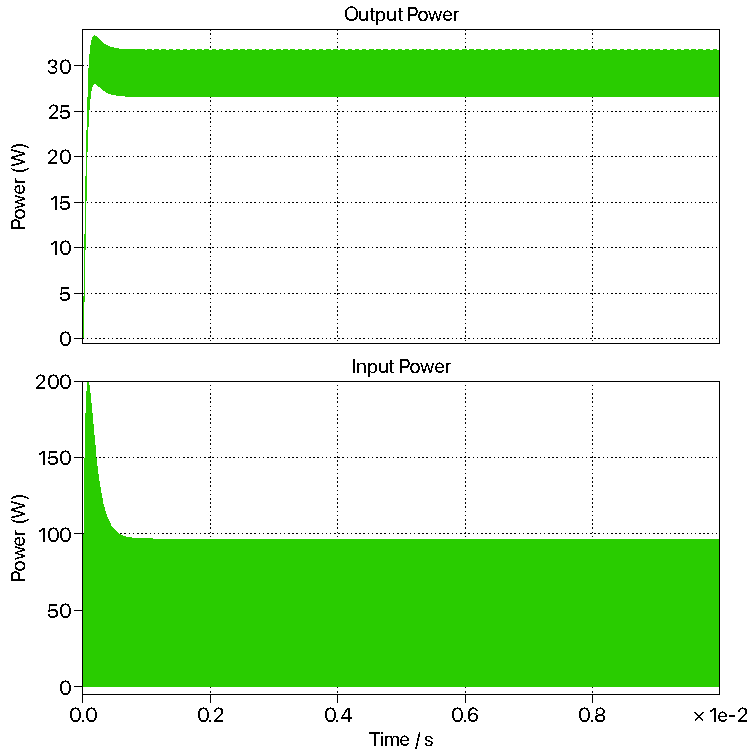
\includegraphics[width=0.6\textwidth]{img/loss-power-bidirectional.pdf}
    \label{fig:loss-bi-plots}
    \caption{Current, Voltage and Power Plot for Bidirectional DC/DC Converter with Losses}
\end{figure}

\subsection{Unidirectional with Losses}

\begin{figure}[H]
    \centering{}
    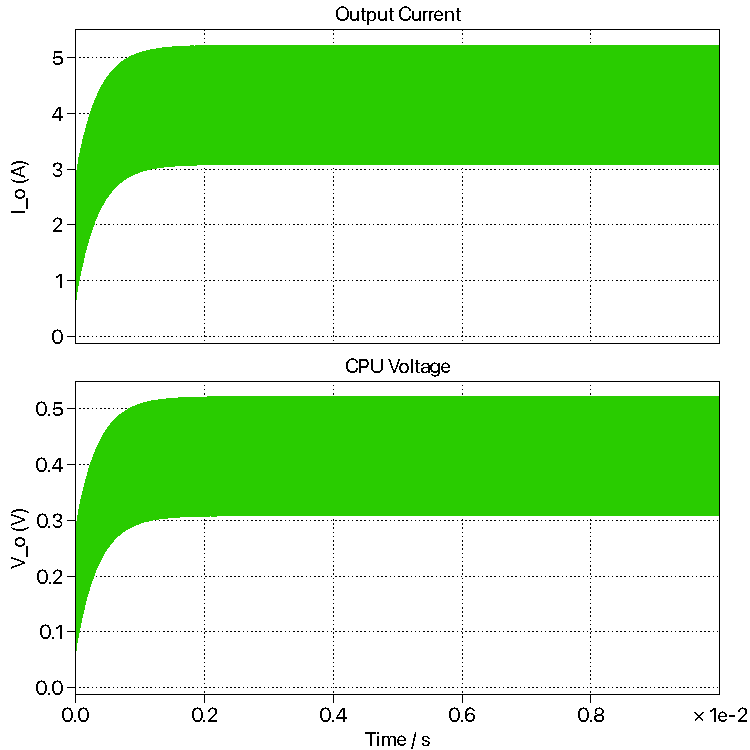
\includegraphics[width=0.6\textwidth]{img/loss-I-V-unidirectional.pdf}
    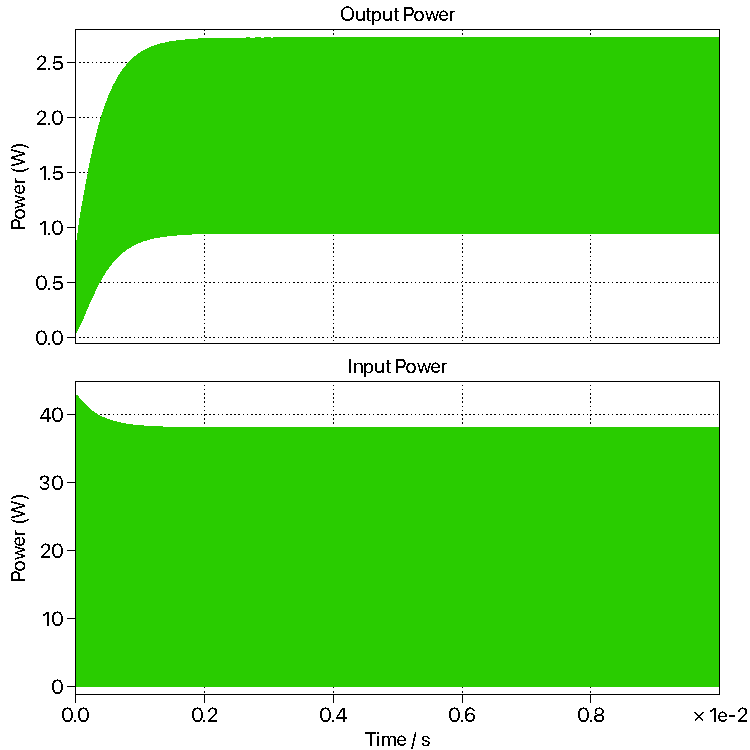
\includegraphics[width=0.6\textwidth]{img/loss-power-unidirectional.pdf}
    \label{fig:loss-uni-plots}
    \caption{Current, Voltage and Power Plot for Unidirectional DC/DC Converter with Losses}
\end{figure}

\section{Power Loss and Efficiency}

This simulation assumes that switching losses for the transistor is negligible (see \ref{subsec:switching-loss}).
Therefore, all the losses are only due to conduction losses.

\begin{table}
    \centering{}
    \label{tab:power-table}
    \caption{Table Detailing Power Characteristics of the Converter}
    \begin{tabularx}{\textwidth}{| X | X | X | X | X |}
        \hline
        Circuit              & Input Power (W) & Output Power (W) & Power Loss (W) & Efficiency (\%) \\
        \hline
        Ideal Bidirectional  & 32.4315         & 32.3953          & 0.0362         & 99.89\%         \\
        Ideal Unidirectional & 32.4387         & 32.3978          & 0.0409         & 99.87\%         \\
        Loss Bidirectional   & 30.8112         & 29.1694          & 1.6418         & 94.67\%         \\
        Loss Unidirectional  & 7.9963          & 1.70261          & 6.29369        & 21.29\%         \\
        \hline
    \end{tabularx}
\end{table}

\subsection{Switching Loss}
\label{subsec:switching-loss}

$P_{SW} = f_s (E_{ON} + E_{OFF} + E_{RR})$

$E_{ON} = \frac{V_{DC} i_{b} t_{ON}}{2} = \frac{5 * 18 * 9e-9}{2} = 0.405 \mu{W}$

$E_{OFF} = \frac{V_{DC} i_{b} t_{OFF}}{2} = \frac{5 * 18 * 21e-9}{2} = 0.945 \mu{W}$

Schottky diodes does not have any reverse recovery losses (in theory). \cite{schotkley-rr-loss}

$E_{RR} = 0 W$

$P_{SW} = 200k (0.405\mu + 0.945\mu) = 76.545 nW$

The switching losses are within nano Watts.
This is negligible compared to the Watts of power generated by the converter.

\section{Differences and Conclusion}

The bidirectional and unidirectional ideal circuit outputs the correct voltage and current value.
The output voltage and inductor current ripple are also within the calculated values at steady state.
However, the bidirectional version returns power during the transient response.
This is due to the bidirectional current flow.

The loss circuits have less current and voltage overshoot.
However, the ripple at steady state are way higher.
Furthermore, the output values have a steady state error.
The efficiency of the loss circuits are also less than the ideal versions.
However, bidirectional efficiency is higher than the unidirectional.
When $G_B$ is low the current flows through the zero loss FET while turned on.
For the unidirectional on the other hand, the current has to flow through the diode which has forward voltage and turn on resistance losses.

The performance of the bidirectional is better than the unidirectional version.
A table comparing their performance is shown in table \ref{tab:comparison}.

\begin{table}[ht]
    \caption{Performance Comparison for Loss Models}
    \label{tab:comparison}
    \begin{tabularx}{\textwidth}{| X | X | X | X | X |}
        \hline
        Circuit        & Current Ripple & Voltage Ripple & Average Current & Average Voltage \\
        \hline
        Expected       & 0.0101 A       & 0.001 V        & 18 A            & 1.8 V           \\
        Unidirectional & 2.13864 A      & 0.21386 V      & 4.05369 A       & 0.406369 V      \\
        Bidirectional  & 1.4995 A       & 0.14995 V      & 17.0708 A       & 1.70708 V       \\
        \hline
    \end{tabularx}
\end{table}

The current design is unacceptable without adding a suitable close loop control system.
The ripple and steady state error makes the converter unusable for any practical applications.
However, once a closed loop control system is designed, the steady state error can be eliminated and the over shoots can be reduced.

\clearpage{}

\printbibliography{}

\clearpage{}

% \section{Appendix}

% 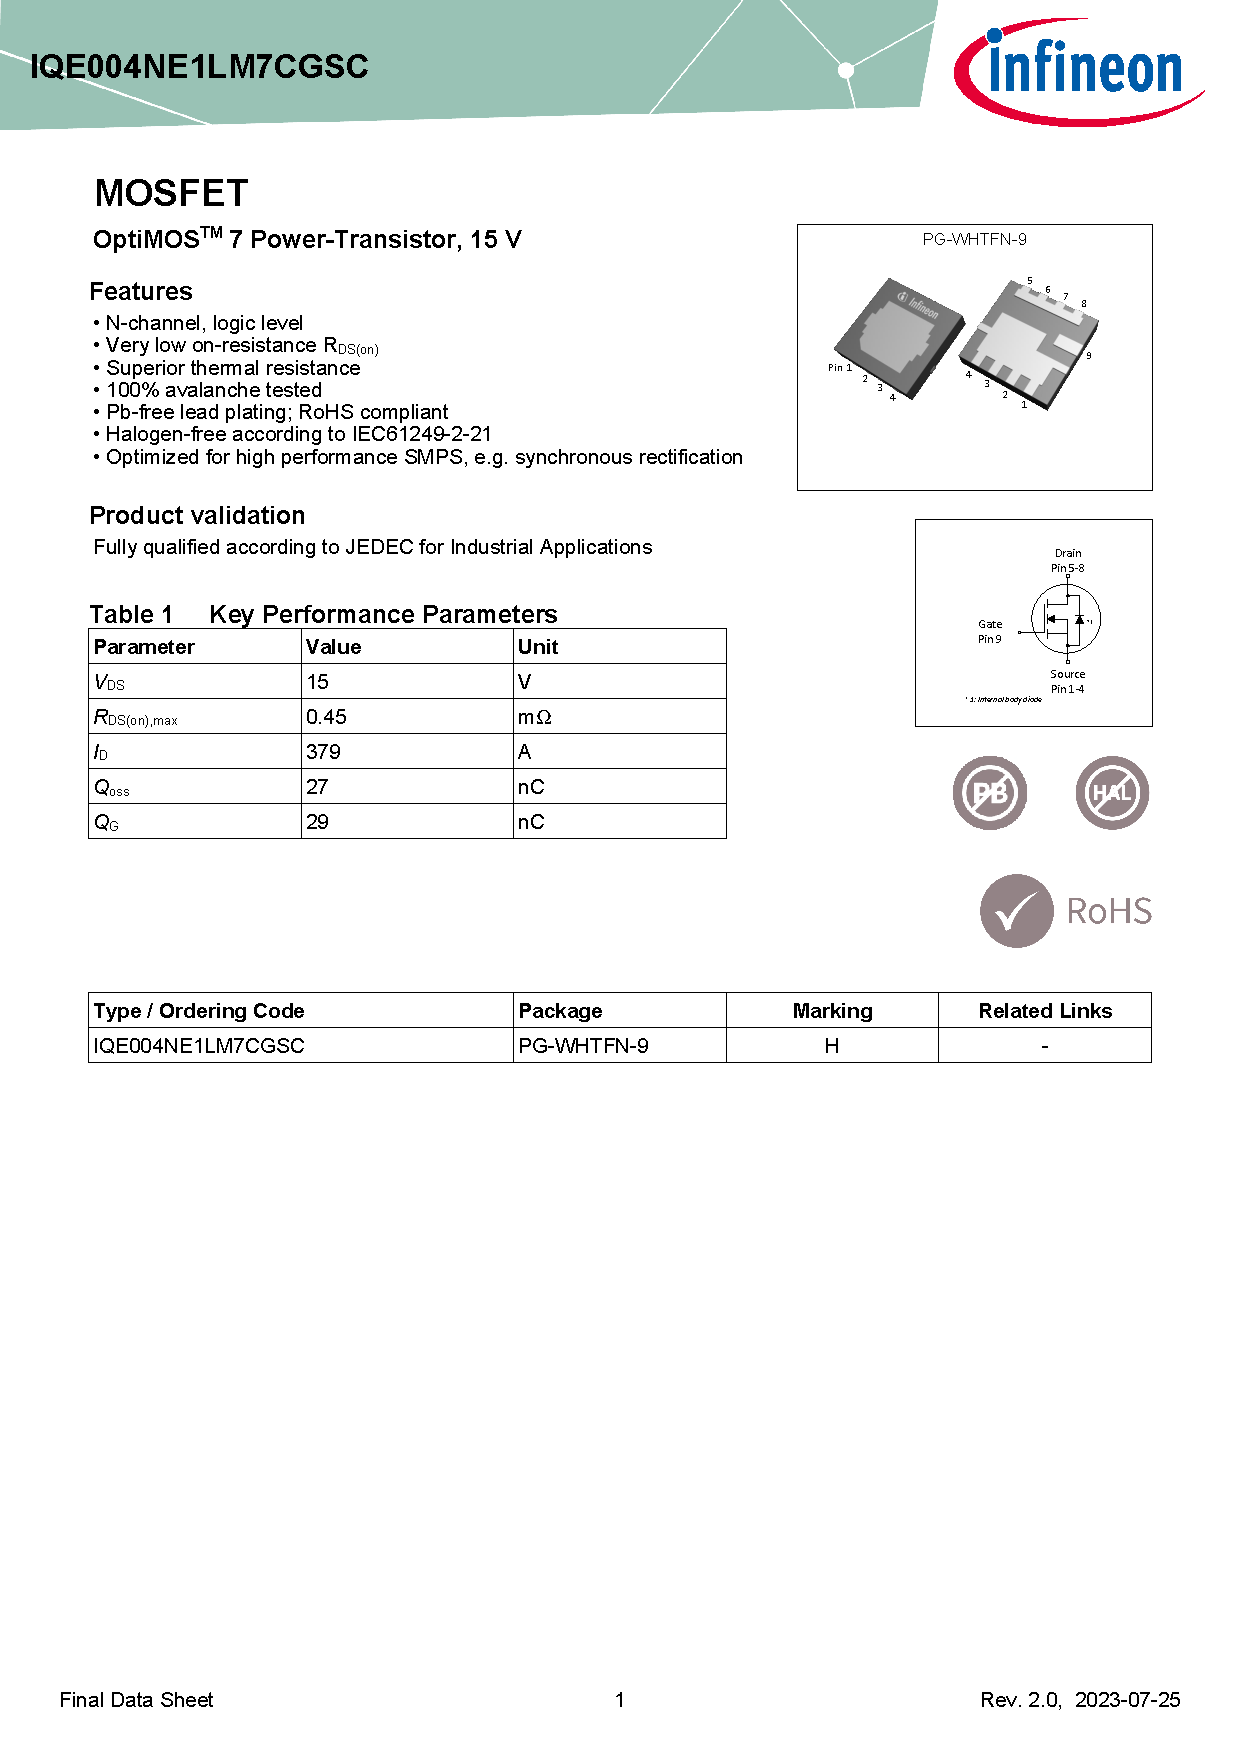
\includepdf{img/Infineon-IQE004NE1LM7CGSC-DataSheet-v02_00-EN.pdf}
% 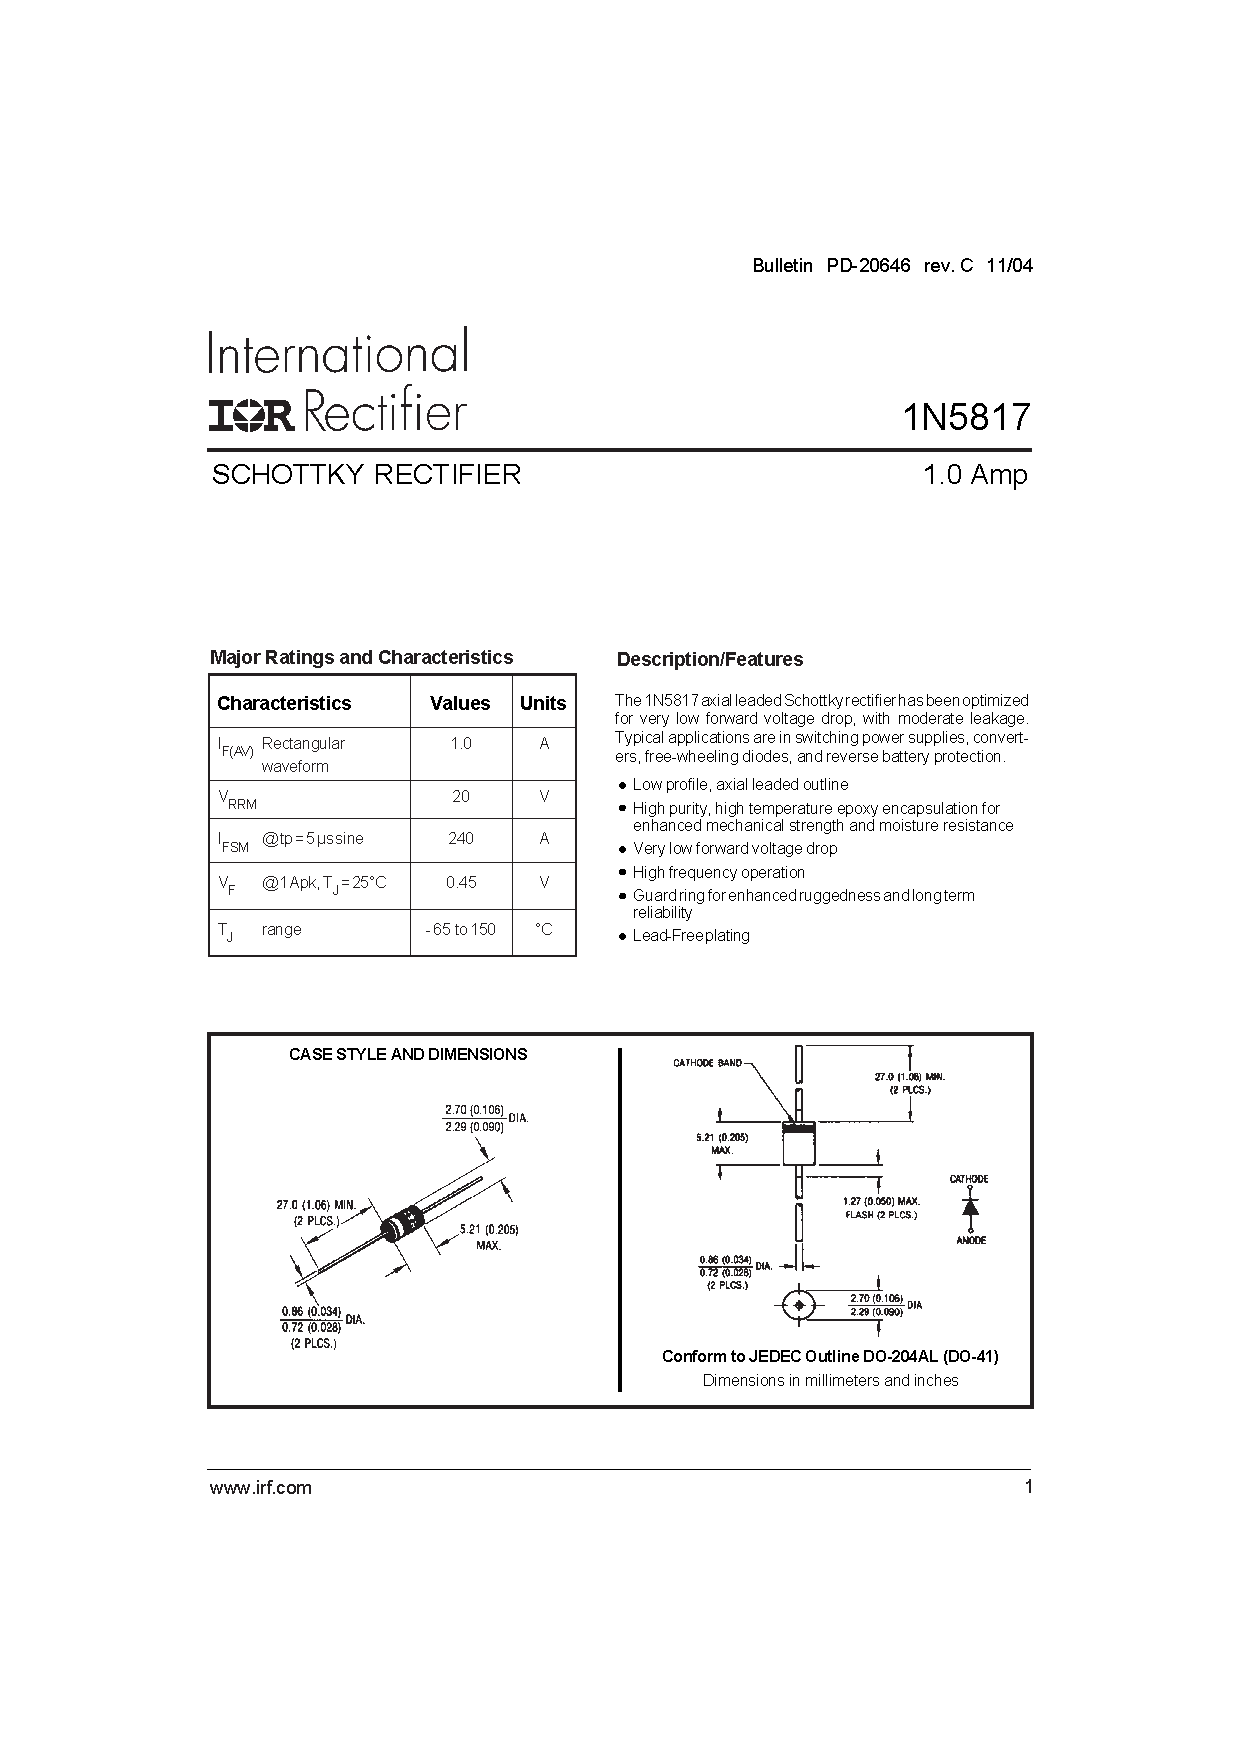
\includepdf{img/1N5817-Schotkey-Diode-Datasheet_0.pdf}

\end{document}
